\documentclass[12pt]{article}
\usepackage{sbc-template}
\usepackage{graphicx,url}
%\usepackage[brazil]{babel}   
\usepackage[utf8]{inputenc}  
\usepackage{makecell}
\usepackage{multirow}
\usepackage{float}
\usepackage{array}
\usepackage{changepage}
\usepackage{enumitem}
\usepackage[normalem]{ulem}
\useunder{\uline}{\ul}{}


\renewcommand{\theenumi}{\Alph{enumi}}

     
\sloppy

\title{Modelos de Classificação de Sentimentos em \emph{Tweets} usando Programação Genética}

\author{Airton Bordin Junior\inst{1}}


\address{Instituto de Informática -- Universidade Federal de Goiás
  (UFG)\\
  Caixa Postal 131 -- 74690-900 -- Goiânia -- GO -- Brazil
}

\begin{document} 

\maketitle

\begin{abstract}
The increase in the number of Internet users in recent years has resulted in a growing content production by its users. Often, the WEB is used as a platform for debates, opinions, evaluations, etc. This fact, in line with the ease of obtaining the information, made the area of Sentiment Analysis, also called Opinion Mining, a growing interest on the part of researchers.

[continue]
\end{abstract}

\begin{resumo} 
O aumento no número de usuários de Internet nos últimos anos teve como consequência uma crescente produção de conteúdo por seus usuários. Frequentemente, a WEB é utilizada como plataforma para debates, opiniões, avaliações, etc. Esse fato, alinhado a facilidade de obtenção dessas informações, fez com que a área de Análise de Sentimentos, também chamada de Mineração de Opiniões, tivesse um interesse crescente por parte de pesquisadores. 

[continuar]
\end{resumo}

\section{Introdução}

A Análise de Sentimentos, também conhecida como Mineração de Opiniões, é uma linha de pesquisa que tem por objetivo a classificação das emoções de um determinado texto, geralmente como positivo, negativo ou neutro. A área vem ganhando destaque nos últimos anos, principalmente por conta da popularização do acesso à Internet e o consequente aumento na quantidade de conteúdo produzido na rede. O uso das redes sociais como \emph{Twitter} e Facebook e a forma com que as pessoas compartilham suas opiniões e sentimentos sobre os mais diversos assuntos tem motivado a pesquisa de formas automatizadas de classificação desses textos.

Podemos dividir as abordagens de classificação de sentimentos em duas classes principais: técnicas supervisionadas e não supervisionadas. A primeira delas utiliza abordagens de aprendizado de máquina para a classificação das opiniões, realizando o treinamento com mensagens previamente classificadas. A abordagem não supervisionada atua em aspectos estruturais do texto e frequentemente fazem uso de Dicionários Léxicos.

Para que um classificador tenha resultados satisfatórios, deve levar em consideração aspectos inerentes do contexto pertencentes às opiniões que serão avaliadas. Um modelo de classificação de \emph{Tweets}, por exemplo, geralmente é diferente de um processo de classificação de avaliações de produtos ou comentários políticos.

A criação de um modelo de classificador de sentimentos de forma manual também depende de conhecimento prévio sobre o domínio a ser analisado, e demanda experiência do projetista, o que pode prejudicar as estratégias e abordagem do sistema.


A programação Genética, explanada em detalhes no seção \ref{progGen}, é uma área da computação evolucionária que busca a criação de modelos para resolver problemas de forma automatizada. Um classificador de sentimentos pode ser visto como um modelo, e a criação de um classificador pode ser abordada como um problema de otimização. Com isso, o presente artigo trabalha com a hipótese que a utilização de Programação Genética apresenta-se como uma alternativa viável para o treinamento e a criação de modelos de classificação de sentimentos eficientes e com resultados satisfatórios.

A proposta principal deste trabalho é a criação de um sistema para a geração de um modelo de classificação de sentimentos, aderente ao contexto para o qual foi treinado, fazendo uso de Programação Genética. 

Algumas questões de pesquisa orientam o desenvolvimento do artigo, e a intenção é que ao final do desenvolvimento do mesmo possamos respondê-las. São elas:

\begin{itemize}
	\item{É possível criar, de forma automatizada, um modelo de classificação de sentimentos utilizando Programação Genética?}
	\item{Caso seja possível, esse modelo é eficiente na classificação de \emph{Tweets} para o contexto que foi criado?}
	\item{Os resultados desse modelo são compatíveis com os classificadores disponíveis atualmente?}
\end{itemize}


A criação de um sistema para a geração automatizada de modelos de classificação de sentimentos, para contextos específicos, e com resultados satisfatórios, pode ser útil para integrar as soluções presentes na literatura e apoiar na validação e na melhoria de modelos já existentes.

Este trabalho está organizado da seguinte maneira: inicialmente, conceitos essenciais para o entendimento do problema de pesquisa são apresentados. Na sequência, a abordagem da solução é apresentada em detalhes. Trabalhos relacionados são discutidos de forma a permitir a comparação do método proposto com outros existentes na literatura. Por fim, os resultados do processo são apresentados.

\section{Conceitos}

Nesta seção, serão apresentados, de forma sucinta, conceitos fundamentais para o entendimento do trabalho. Pontos principais dos temas serão discutidos, com foco nos conceitos relevantes para a solução do problema de pesquisa.

\subsection{Análise de Sentimentos}
A Análise de Sentimentos, também chamada de Análise de Opiniões ou Mineração de Opiniões, é uma linha de pesquisa abrangente e que vem sendo tema de diversos trabalhos nos últimos anos. Como observado em \cite{liu2010multifaceted}, esse crescente interesse sobre o assunto ocorre principalmente devido ao aumento no número de usuários de Internet e o consequente crescimento da produção de conteúdo independente na rede, como opiniões, avaliações, entre outros. 

Essa área de estudo tem como principal desafio a Análise de Opiniões, descritas em linguagem natural, para a identificação da polaridade implícita ou explícita no texto. Essa polaridade é, na maior parte das vezes, identificada como uma escala de pontuação de sua característica positiva, negativa ou neutra.

Quanto aos classificadores de sentimentos, há duas formas principais para o processamento e classificação das mensagens: a abordagem supervisionada e não supervisionada. Na abordagem supervisionada, técnicas de aprendizado de máquina são aplicados à mensagens previamente rotuladas de forma a identificar características que auxiliem na distinção e detecção de sentimentos nas sentenças desconhecidas. Técnicas não supervisionadas atuam principalmente em características sintáticas e semânticas do texto e, geralmente, baseiam-se em Dicionários Léxicos - conjunto de palavras e suas polaridades (grau de positividade e negatividade de uma mensagem). À partir desse dicionário, é feito o processamento das mensagens pelo classificador e retornada a polaridade da mesma. \cite{araujo2013metodos}

Dentre as principais técnicas de aprendizado de máquina para a classificação de sentimentos, podemos citar o \emph{Support Vector Machines} (SVM) \cite{HADDI2013}, \emph{Naïve Bayes} \cite{Iqbal}, \emph{Adaboost} \cite{graff2017semantic}, Redes Neurais Artificiais, entre outros. \cite{Rodrigues2016}

Importante destacar que, para o desenvolvimento de um bom modelo supervisionado, é essencial que haja uma quantidade considerável e representativa de dados previamente rotulados pertencentes ao domínio do problema, para que o treinamento possa ser feito de forma satisfatória. \cite{araujo2013metodos}

As abordagens não supervisionadas baseadas em Léxico, como discutido anteriormente, fazem uso de um conjunto de palavras e suas polaridades. Alguns classificadores utilizam Dicionários Léxicos já existentes, enquanto outros se encarregam de criar o próprio dicionário, mais adequado ao contexto e domínio da análise. Essa estratégia faz uso das características do texto e regras sintáticas para determinar a classificação de palavras e frases desconhecidas à partir das palavras contidas no dicionário e suas relações. Dentre as principais técnicas dessa categoria podemos citar \emph{Part-of-Speech Tag} \cite{becker2013}, \emph{Pointwise Mutual Infomation} (PMI) \cite{Turney2002}, entre outros.

Para técnicas que se encarregam da criação e expansão do próprio Dicionário Léxico há, basicamente, 3 formas de fazê-lo: manualmente -  processo realizado por especialistas humanos que analisam cada palavra, atribuindo uma Orientação Semântica para cada uma delas -  e duas formas (semi) automatizadas: baseada em Dicionário e baseada em Corpus. Frequentemente, essas técnicas são utilizadas em conjunto, principalmente a validação manual de Dicionários criados de forma automatizada.

O contexto no qual uma palavra está inserida muitas vezes determina seu valor na classificação da opinião como um todo. Palavras pode ter polaridades diferentes, dependendo do domínio ao qual é aplicada. Sabendo disso, classificadores de sentimentos devem levar em consideração uma série de fatores para que os resultados da mineração de opiniões seja satisfatório. Não há um modelo pré definido para a classificação de sentimentos em qualquer contexto.

\subsection{Programação Genética}
\label{progGen}
Programação Genética é um campo da computação evolucionária que busca resolver problemas, de forma automatizada, sem demandar conhecimentos detalhados sobre a solução \cite{koza1992genetic}. De forma geral, podemos definir a Programação Genética como um método sistemático, não dependente de um domínio específico, usado para permitir que computadores criem programas para solução de problemas de forma automática, inciando com um conhecimento de alto nível sobre as regras gerais dos possíveis modelos.

Nesse contexto, programa significa um modelo capaz de, à partir de uma ou mais entradas, produzir uma saída para as mesmas. Embora possam ser representadas por diversos tipos de estruturas, a forma mais comum de representação é por meio de árvores, onde os nós internos representam funções e os nós folha representam terminais do problema. Um exemplo de um programa pode ser visto na figura \ref{treeProgram}, que representa o código \emph{if( X \textgreater Y) then \{ X * 6 +  1.9 \} else \{ X / cos(X) \}}

\begin{figure}[!htb]
	\centering
	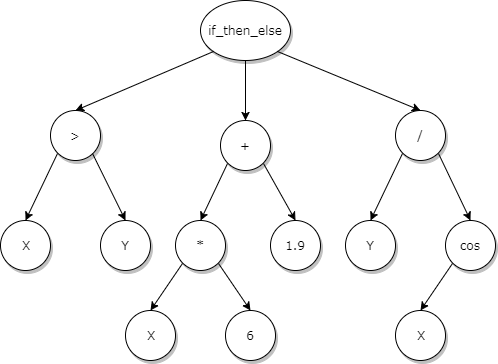
\includegraphics[width=0.7\textwidth]{treeGP}
	\caption{Exemplo de um programa em Programação Genética}
	\label{treeProgram}
\end{figure}

Na Programação Genética, assim como em outros algoritmos baseados na evolução humana, são criadas populações onde cada indivíduo representa uma possível solução para o problema. A forma mais comum de inicialização da população é fazê-las de forma aleatória, evoluindo as mesmas no decorrer dos ciclos, chamados de gerações. Para cada geração, programas possivelmente melhores são criados, evoluindo os programas (modelos) gerados. Assim como a natureza, a Programação Genética é um processo aleatório, e não garante o resultado ótimo. Porém, essa aleatoriedade faz com que, muitas vezes, as soluções fujam de problemas como soluções máximas locais, frequentemente enfrentados por métodos determinísticos gulosos \cite{mcphee2008field}.

Uma das características mais importantes da Programação Genética é a função de aptidão, ou função \emph{fitness}. Essa função busca representar, de forma quantitativa, a similaridade de cada indivíduo em relação ao resultado esperado. A escolha de uma boa função \emph{fitness} está intimamente ligada ao tipo do problema.

Os responsáveis pela evolução da população de indivíduos são os operadores genéticos. Para a Programação Genética, os principais operadores são a seleção, mutação e \emph{crossover}. Na seleção, um indivíduo é escolhido para fazer parte da próxima geração. A mutação modifica um nó da árvore, de forma a criar um indivíduo modificado em uma das partes escolhida aleatoriamente. O \emph{crossover} realiza o cruzamento entre dois indivíduos (pais), gerando duas novas possíveis soluções para o problema (filhos). Além desses principais operadores, existem outros como a edição, encapsulamento e a destruição \cite{patelli2011genetic}.

Por sua característica inerentemente paralela, esse tipo de abordagem consegue encontrar resultados muito próximos da solução ótima (às vezes encontra a melhor resolução) para problemas complexos com grandes espaços de busca.

\section{Trabalhos relacionados}

\label{sec:bibl}

Como discutido em seções anteriores, a quantidade de trabalhos na área de análise de sentimento vem crescendo a cada ano, motivado, principalmente, pela importância da área no contexto atual de geração e análise de grande quantidade de dados e informações.

Ao debatermos os trabalhos relacionados à área de mineração de opiniões, é praticamente impossível não iniciarmos citando \cite{liu2010multifaceted}, uma das principais referências do assunto. O autor, um dos principais nomes sobre o assunto, conceitualiza o problema e propõe uma forma estruturada de organização dos dados não estruturados, característica instrínseca dos textos em linguagem natural, objeto de entrada da pesquisa. A definição de opinião como uma quíntupla (entidade, aspecto da entidade, sentimento, autor e tempo) é utilizada em grande parte dos trabalhos na área, caracterizando-se, portanto, como elemento fundamental nas pesquisas sobre o assunto. Visão geral sobre o tema e principais desafios e técnicas são vistos também em \cite{mohammad2016challenges}, \cite{ghaleb2016survey}, \cite{kdir16}, \cite{taboada2011lexicon}, \cite{bandhakavi2016lexicon}, \cite{Alessia}, \cite{kaji}, entre outros trabalhos.

Embasamento teórico sobre a divisão dos métodos de classificação de sentimentos em abordagens supervisionadas e não supervisionadas são apresentadas de forma clara em \cite{araujo2013metodos}

No contexto de prognóstico automatizado de Orientação Semântica de palavras, um dos primeiros trabalhos apresentados foi \cite{Hatzivassiloglou}, focando na previsão de polaridade de adjetivos.

Uma das formas não supervisionadas de classificação leva em consideração aspectos sintáticos e semânticos do texto. \cite{Turney2002} apresenta uma abordagem de expansão léxica fazendo uso da técnica de \emph{Pointwise Mutual Infomation} (PMI), com o objetivo de calcular a coocorrência de palavras e, com isso, comparar a polaridade de novas palavras com outras já conhecidas. Nesse trabalho, amplamente referenciado por outras pesquisas, o autor compara o conjunto de palavras de Orientação Semântica desconhecida com as palavras \emph{ "excellent"} e \emph{"poor"}, representando Orientações Semânticas positiva e negativa, respectivamente. Essas palavras previamente conhecidas utilizadas como base para a expansão do Dicionário são chamadas de palavras semente (\emph{seed words}, em inglês). Como exemplo de trabalhos que utilizam o PMI para a criação e expansão do Dicionário Léxico podemos citar \cite{becker2013}, \cite{Zhou2014}, \cite{Pinto2007}. \cite{Pantel2006}, \cite{duwairi2015detecting}, entre outros.

Outro importante trabalho sobre Mineração de Opiniões, \cite{taboada2011lexicon} apresenta uma abordagem de Análise de Sentimentos baseada em Léxico combinada com uma verificação manual. Esse trabalho apresenta o SO-CAL (\emph{Semantic Orientation Calculator}), que usa lista de palavras já consolidadas para a geração de dicionários com novas entradas e suas polaridades de forma não supervisionada.

Na linha de estratégias supervisionadas, \cite{eisenstein2016unsupervised} e \cite{bandhakavi2016lexicon} apresentam outros procedimentos para apoiar a Análise de Sentimentos. O primeiro apresenta uma abordagem usando a técnica de \emph{Naive Bayes} para a classificação dos aspectos e cita problemas de estimativas de palavras e avaliação dos léxicos criados. O segundo faz uma comparação de algumas técnicas de avaliação em 4 conjuntos de dados diferentes, apresentando uma análise quantitativa do mesmo. Abordagens e comparações semelhantes, com algumas modificações no domínio e no idioma do problema abordado, podem ser vistos em \cite{khoo2017lexicon}, \cite{asghar2014review} e \cite{ding2008holistic}.

Sistemas Classificadores, como o criado em \cite{Rodrigues2016}, recebem como entrada um texto e retornam a Orientação Semântica do mesmo. Para esse processo, \cite{Rodrigues2016} faz uso de um Dicionário próprio, com grande parte das polaridades anotadas manualmente. O processo de classificação, desafios da área e outros exemplos de classificadores são discutidos em \cite{Pang2002}, \cite{Zhou2014}, \cite{silva2010automatic}, \cite{kdir16}, entre outros.

Importante destacar, como bem apresentado por \cite{araujo2013metodos}, que somente o Dicionário Léxico não é capaz de prover uma classificação dos sentimentos eficaz e a simples soma das polaridades das palavras pode apresentar resultados não satisfatórios, levando a uma avaliação incorreta. Grande parte dos classificadores possuem heurísticas que trabalham em conjunto com os dicionários, além de processamentos prévios das mensagens, o que proporciona um melhor resultado das classificações.

De forma geral, essas estratégias heurísticas levam em consideração aspectos gramaticais e sintáticos que tem possuem uma importância na expressão do sentimento, como pontuação, negação, intensificação, capitalização, entre outros. Em contextos específicos, como a classificação de \emph{Tweets}, pode-se levar em consideração a quantidade de \emph{hashtags}, gírias, etc.

A criação de modelos pode ser vista como um problema de otimização. Para essa classe de problemas, podemos fazer uso de estratégias de computação evolucionária, baseadas na teoria da evolução de \emph{Darwin}. Dentre os trabalhos que abordam a Análise de Sentimentos fazendo uso de Estratégias Evolutivas, podem citar \cite{ferreira2015using}, \cite{vohra2013comparative}, \cite{HADDI2013} e \cite{silveirageraccao}.

Conjuntos de dados previamente avaliados são amplamente utilizados para teste dos Sistemas de Classificação. Esses dados tem sua Orientação Semântica determinadas por especialistas humanos, e servem como entrada para a comparação da saída dos classificadores, ou seja, são dados considerados corretos e consistentes. Principais conjuntos de dados disponíveis para utilização no processo de Análise de Sentimentos podem ser vistos em \cite{HuAndLiu2004}, \cite{Iqbal}, \cite{taboada2011lexicon}, entre outros. 


\section{Abordagem}
Nesta seção, serão apresentadas as abordagens de análise do problema de pesquisa e do projeto da solução, com detalhes relevantes de implementação, dados utilizados, bibliotecas de apoio, entre outros.

\subsection{Análise do problema}

A criação de um classificador de sentimentos para um determinado contexto é um desafio de pesquisa na área de Análise de Sentimentos. Detalhes intrínsecos do domínio do texto, idioma, entre outros, podem ser relevantes para as regras de classificação. 

O modelo de classificação, portanto, pode ser descrito como um programa. Podemos abordar essa situação como um problema de otimização, com o objetivo de encontrar um modelo que represente a solução desejada.

A Programação Genética pode auxiliar nesse processo de criação do modelo de classificação. De posse de um conjunto de dados previamente classificados, podemos treinar nossa população de possíveis soluções (indivíduos), avaliando seu \emph{fitness} de acordo com a semelhança com o resultado esperado para determinada entrada.

Por possuir uma forma de atuação paralela, essa abordagem resulta em soluções muito próximas da solução ótima (às vezes encontra a melhor resolução) para problemas complexos.

O indivíduo mais apto (de melhor \emph{fitness}) retornado pelo algoritmo de Programação Genética tem grandes chances de ser um modelo de classificação de sentimentos com bons resultados.

\subsection{Projeto da solução}

Como explanado na seção \ref{progGen}, a Programação Genética pode ser utilizada para a criação de um modelo de solução - um programa - para a resolução de um dado problema. No caso do presente trabalho, queremos encontrar um modelo de classificação de sentimentos em \emph{Tweets}.

O primeiro passo para projetar uma solução de Programação Genética é determinar o conjunto de terminais e funções do modelo. Os terminais serão compostos pelos \emph{Tweets} que serão analisados, bem como por uma constante efêmera, um número real escolhido aleatoriamente entre -3 e 3. A constante efêmera será escolhida de forma aleatória somente no momento de criação do indivíduo, e depois manterá seu valor na árvore.

As funções serão responsáveis por realizar a manipulação dos dados, como o \emph{Tweet} e suas características. A lista das principais funções definidas para a solução pode ser vista na tabela \ref{tab_functions}.


Para a criação das funções, foi levado em consideração heurísticas apresentadas em trabalhos anteriores sobre o tema e para determinados contextos, como os apresentados em \cite{araujo2013metodos}, \cite{Rodrigues2016}, \cite{Turney2002}, entre outros.

\begin{table}[H]
	\centering
	\begin{tabular}{ll}
	\multicolumn{1}{c}{\textbf{Função}} & \multicolumn{1}{c}{\textbf{Retorno}} \\
	\hline
	polaritySum(str): float & Soma das polaridades de cada palavra  \\
	\hline
	hashtagPolaritySum(str): float & Soma das polaridades de cada hashtag \\
	\hline
	emoticonPolaritySum(str): float & Soma das polaridades de cada emoticon  \\
	\hline
	positiveWordsQuantity(str): float & Quantidade de palavras positivas \\
	\hline
	negativeWordsQuantity(str): float & Quantidade de palavras negativas \\
	\hline
	hasHashtags(str): bool & Verifica se o \emph{Tweet} possui hashtag \\
	\hline
	hasEmoticons(str): bool & Verifica se o \emph{Tweet} possui emoticon \\
	\hline
	removeStopWords(str): str & Remove os \emph{stopwords} do \emph{Tweet} \\
	\hline
	\end{tabular}
	\caption{Principais funções utilizadas na Programação Genética}
	\label{tab_functions}
\end{table}

Além das funções citadas na tabela \ref{tab_functions}, também foram incluídas funções matemáticas como adição, subtração, divisão, multiplicação, logaritmo, raiz quadrada, exponenciação, seno e cosseno.

Outra característica importante a ser definida para o trabalho é a função de \emph{fitness}. Para a solução, o \emph{fitness} é definido como o F1 médio do classificador, calculado utilizando a fórmula apresentada na tabela \ref{metrics}

\begin{table}[H]
\centering
	\begin{tabular}{ll}
	\multicolumn{1}{c}{\textbf{Terminologia}} & \multicolumn{1}{c}{\textbf{Descrição}} \\ \hline
	Verdadeiro Positivo (VP) & Modelo retornou Positivo e a classe real é Positivo \\ \hline
	Verdadeiro Negativo (VN) & Modelo retornou Negativo e a classe real é Negativo \\ \hline
	Verdadeiro Neutro (VNt) & Modelo retornou Neutro e a classe real é Neutro \\ \hline
	Falso Positivo (FP) & Modelo retornou Positivo e a classe real não é Positivo \\ \hline
	Falso Negativo (FN) & Modelo retornou Negativo e a classe real não é Negativo \\ \hline
	Falso Neutro (FNt) & Modelo retornou Neutro e a classe real não é Neutro \\ \hline
	\end{tabular}
	\caption{Dados utilizados para as métricas do modelo}
	\label{metricsTrueFalse}
\end{table}

Outras métricas são utilizadas para a verificação da qualidade do classificador: acurácia, precisão e \emph{recall}. Detalhes de cada uma dessas funções são apresentadas na tabela \ref{metrics}. Para todas essas medições, são considerados 6 possibilidades de classificação dos \emph{Tweets}: Verdadeiro Positivo (VP), Verdadeiro Negativo (VN), Verdadeiro Neutro (VNt), Falso Positivo (FP), Falso Negativo (FN) e Falso Neutro (FNt), conforme apresentado na tabela \ref{metricsTrueFalse}.


\begin{table}[H]
\centering
	\begin{tabular}{ll}
	\multicolumn{1}{c}{\textbf{Métrica}} & \multicolumn{1}{c}{\textbf{Fórmula}} \\ \hline
	Acurácia & (VP + VN + VNt )/ Total de mensagens \\ \hline
	Precisão positiva (PP) & VP / Positivos retornados pelo modelo \\ \hline
	\textit{Recall} positivo (RP) & VP / Mensagens positivas \\ \hline
	F1 positivo (FP) & 2 x (PP * RP) / (PP + RP) \\ \hline
	Precisão negativa (PN) & VN / Negativos retornados pelo modelo \\ \hline
	\textit{Recall} negativo (RN) & VN / Mensagens negativas \\ \hline
	F1 negativo (FN) & 2 x (PN * RN) / (PN + RN) \\ \hline
	Precisão neutra (PNt) & VNt / Neutros retornados pelo modelo \\ \hline
	\textit{Recall} neutro (RNt) & VNt / Mensagens neutras \\ \hline
	F1 neutro (FNt) & 2 x (PNt * RNt) / (PNt + RNt) \\ \hline
	Precisão média & (PP + PN + PNt) / 3 \\ \hline
	\emph{Recall} médio & (RP + RN + RNt) / 3 \\ \hline	
	F1 médio & (FP + FN + FNt) / 3 \\ \hline
	F1 médio SemEval & (FP + FN) / 2 \\ \hline	
	\end{tabular}
	\caption{Métricas utilizadas para avaliar o modelo de classificação}
	\label{metrics}
\end{table}

\subsection{Bibliotecas}

Para apoiar no desenvolvimento da solução do problema, foi utilizada a biblioteca DEAP\footnote{https://github.com/DEAP/deap} (\emph{Distributed Evolutionary Algorithms in Python}), escrita na linguagem \emph{Python} e disponível para uso gratuito. Fornece abstrações para a implementação de várias classes de algoritmos evolucionários, como Algoritmos Genéticos, Programação Genética, entre outros. \cite{DEAP_JMLR2012}

Especificamente para o contexto de Programação Genética, DEAP fornece funcionalidades para controle de criação das estruturas de árvores, operadores genéticos, parametrização das operações, \emph{logs}, entre outras.

\subsection{Dicionários}

Para o presente trabalho, foram utilizados os dicionários de palavras positivas e negativas de \cite{HuAndLiu2004}\footnote{https://www.cs.uic.edu/~liub/FBS/sentiment-analysis.html\#lexicon}. Os dicionários fornecem um conjunto de 4783 palavras negativas e 2006 palavras positivas para apoiar no processo de Análise de Sentimentos.

Utilizou-se, também, o dicionário de \emph{emoticons} SentiStrength\footnote{http://sentistrength.wlv.ac.uk/}, que fornece 46 \emph{emoticons} positivos e 58 negativos.

A escolha desses dicionários deu-se, principalmente, por terem sido utilizados como base para o SemEval 2014, \emph{task} 9. Ao considerar as mesmas bases disponibilizadas pela competição, é possível fazer a comparação dos resultados obtidos neste trabalho com os avaliados pelo evento.

\subsection{\emph{Datasets}}
\label{datasets}
Há diversas bases de dados anotadas disponíveis na Internet para \emph{download}. O escopo do presente trabalho é a Análise de Sentimentos em \emph{Tweets}, por isso utilizou-se uma base disponibilizada para o evento SemEvaL 2014\footnote{http://alt.qcri.org/semeval2014/} (\emph{International Workshop on Semantic Evaluation}), uma das principais referências na área de análise semântica.  

O evento é dividido por \emph{Tasks}, que possuem objetivos distintos dentro da área de pesquisa. Para este trabalho, utilizou-se a base de dados da \emph{Task 9} - \emph{Sentiment Analysis in Twitter}. São disponibilizadas bases de treinamento e de testes para \emph{download}\footnote{http://alt.qcri.org/semeval2014/task9/index.php?id=data-and-tools} no site do evento.

A base de treinamento aplicada no trabalho possui 9684 \emph{Tweets}, com a seguinte divisão de polaridades: 3640 mensagens positivas, 1458 negativas e 4586 neutras.

\begin{figure}[H]
	\centering
	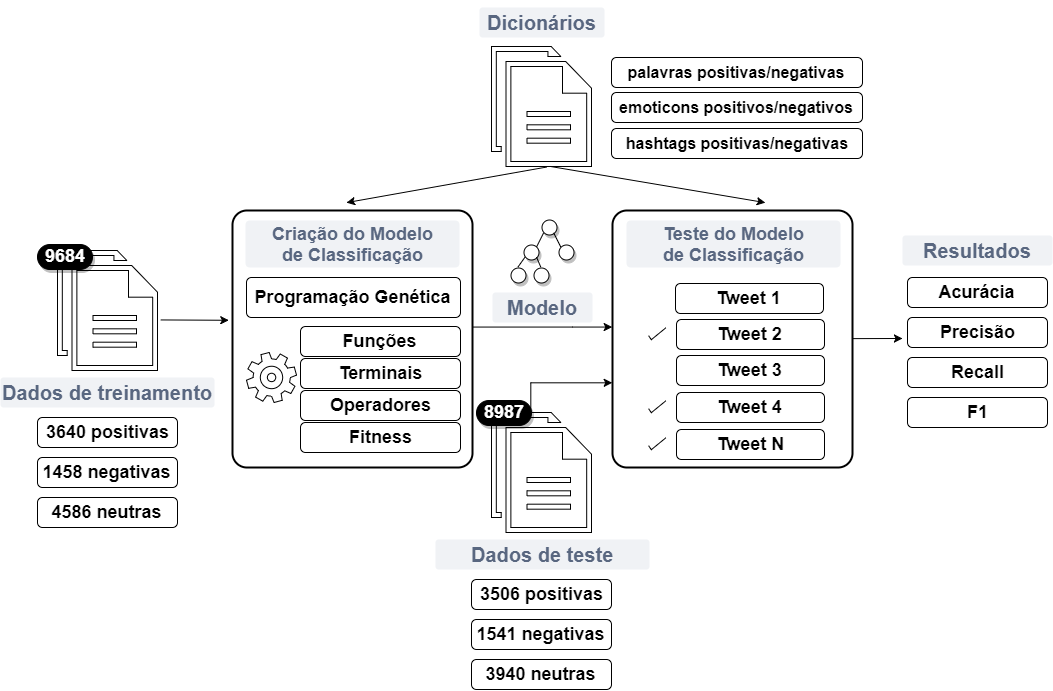
\includegraphics[width=1\textwidth]{diagrama3}
	\caption{Diagrama simplificado da solução}
	\label{diagrama}
\end{figure}

O evento também disponibiliza uma base de testes, que serve como critério de avaliação e comparação dos trabalhos submetidos para cada \emph{task}. A base fornecida é dividida em 5 categorias, e possui um total de 8987 \emph{Tweets}. Detalhes da divisão e da polaridade das bases podem ser visualizadas na tabela \ref{datasets}.

\begin{table}[H]
\centering
	\begin{tabular}{lc}
	\multicolumn{1}{c}{\textbf{Base de Dados}} & \textit{\textbf{Tweets}} \\ \hline
	Tweets2013 & 3813 \\ \hline
	Tweets2014 & 1853 \\ \hline
	\textit{Tweets2014Sarcasm} & 86 \\ \hline
	SMS2013 & 2093 \\ \hline
	LiveJournal2014 & 1142 \\ \hline
	Total & 8987 \\ \hline
	\end{tabular}
\caption{Bases de testes - Semeval2014}
\label{datasets}
\end{table}

\section{Resultados}

Nesta seção, serão apresentados os resultados obtidos com os modelos gerados pelo sistema. 

\subsection{Criação do modelo}

A criação do modelo é feita pelo processo de Programação Genética, tendo como entrada os \emph{Tweets} da base de treinamento utilizada no trabalho e discutida na seção \ref{datasets}. Os processos de Programação Genética encarregam-se da criação e evolução da população de indivíduos, conforme os princípios citados anteriormente.

Alguns parâmetros devem ser definidos para o funcionamento da Programação Genética. Os principais deles são quantidade de gerações, população, taxa de \emph{crossover} e taxa de mutação. Não há uma regra para a definição desses valores, e cada problema deve ter uma abordagem diferente. Para o presente trabalho, os parâmetros definidos para a criação e evolução dos modelos podem ser vistos na tabela \ref{parametersGP}.

\begin{table}[H]
	\centering
	\begin{tabular}{cccccc}
	\textbf{Modelo} & \textbf{População} & \textbf{Gerações} & \textbf{\emph{Crossover}} & \textbf{Mutação} & \textbf{Gerações sem evolução} \\ \hline
	A & 50 & 500 & 3.5\% & 1.5\% & 150 \\ \hline
	B & 50 & 600 & 9.5\% & 5.5\% & 300 \\ \hline
	C & 100 & 500 & 4.5\% & 2.5\% & 500 \\ \hline
	\end{tabular}
	\caption{Parâmetros da Programação Genética}
	\label{parametersGP}
\end{table}

Com o objetivo de diminuir a quantidade de tempo de processamento para a criação dos modelos pelo algoritmo de Programação Genética, foi criado um parâmetro que determina a quantidade máxima aceitável de gerações sem evolução no \emph{fitness}, ou seja, a quantidade de ciclos seguidos em que não houve melhoria no melhor indivíduo da população. 

Inicialmente, foram criados 3 modelos de classificação de sentimentos, usando as mesmas entradas (base de treinamento) e modificando somente os parâmetros da Programação Genética. Cada um dos modelos foi testado com a base de testes disponibilizada pelo SemEval 2014.

Os modelos criados após o processamento foram (a variável x representa a entrada, nesse caso, os \emph{Tweets}):

	\begin{figure}[H]
		\centering
		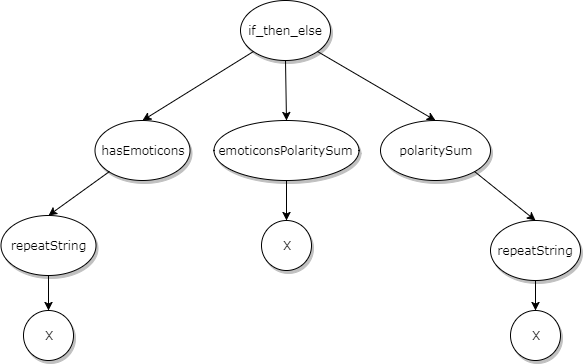
\includegraphics[width=0.9\textwidth]{treeA}
		\caption{Modelo A}
		\label{AModel}
	\end{figure}
	
	\begin{figure}[H]
		\centering
		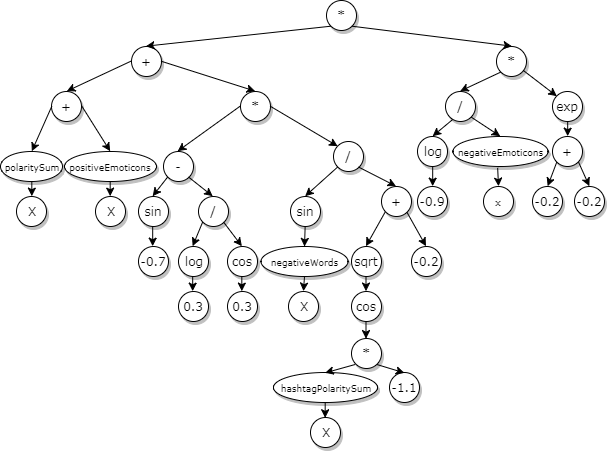
\includegraphics[width=1.0\textwidth]{treeB2}
		\caption{Modelo B}
		\label{BModel}
	\end{figure}

	\begin{figure}[H]
		\centering
		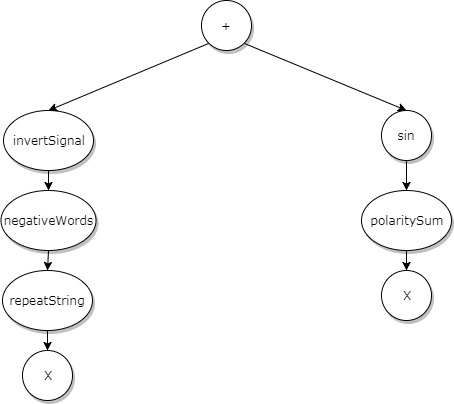
\includegraphics[width=0.75\textwidth]{treeC}
		\caption{Modelo C}
		\label{CModel}
	\end{figure}




\subsection{Testes dos modelos}

Os modelos foram testados com a base de testes disponibilizada pela organização do evento SemEval 2014. Como apresentado na tabela \ref{datasets}, as mensagens são divididas em 5 bases de teste: Twitter2013, Twitter2014, Twitter2014Sarcasm, SMS2013 e LiveJournal2014. Os resultados foram calculados para cada base e, posteriormente, de forma geral, utilizando todas as mensagens.

A tabela \ref{correctEvaluations} apresenta a quantidade de \emph{Tweets} avaliados corretamente por modelo. 

\begin{table}[H]
\centering
\begin{adjustwidth}{-1.5cm}{}
\begin{tabular}{lccccccccccccc}
\multicolumn{1}{c}{\textbf{Base}} & \textit{\textbf{Tweets}} & \multicolumn{12}{c}{\textbf{Avaliados corretamente}} \\
 & \multicolumn{1}{l}{} & \multicolumn{4}{c}{Modelo A} & \multicolumn{4}{c}{\textbf{Modelo B}} & \multicolumn{4}{c}{Modelo C} \\
 & \multicolumn{1}{l}{} & \multicolumn{1}{c|}{P} & \multicolumn{1}{c|}{N} & \multicolumn{1}{c|}{Nt} & T & \multicolumn{1}{c|}{P} & \multicolumn{1}{c|}{N} & \multicolumn{1}{c|}{Nt} & T & \multicolumn{1}{c|}{P} & \multicolumn{1}{c|}{N} & \multicolumn{1}{c|}{Nt} & T \\
Tweets2013 & 3813 & 779 & 239 & 1257 & 2275 & 773 & 279 & 1253 & 2287 & 674 & 294 & 1261 & 2229 \\ \hline
Tweets2014 & 1853 & 425 & 69 & 507 & 1001 & 422 & 79 & 494 & 995 & 354 & 85 & 503 & 942 \\ \hline
Sarcasm & 86 & 11 & 2 & 11 & 24 & 11 & 3 & 11 & 25 & 11 & 5 & 11 & 27 \\ \hline
SMS2013 & 2093 & 237 & 120 & 993 & 1350 & 234 & 135 & 986 & 1355 & 209 & 136 & 999 & 1344 \\ \hline
LiveJournal & 1142 & 257 & 131 & 312 & 700 & 255 & 154 & 307 & 716 & 233 & 157 & 314 & 704 \\ \hline
Todas & 8987 & 1709 & 561 & 3080 & 5350 & 1695 & 650 & 3033 & 5378 & 1481 & 677 & 3088 & 5246\\ \hline
\end{tabular}
\caption{Avaliações corretas por base}
\label{correctEvaluations}
\end{adjustwidth}
\end{table}


Com relação ao cálculo de outras métricas (apresentadas na tabela \ref{metrics}), especificamente no processamento de F1, foi criada uma segunda média, levando em consideração somente o F1 positivo e negativo, desconsiderando o neutro. Esse foi o critério adotado pela equipe de avaliação do SemEval 2014 (\emph{task} 9, B), e foi aplicado no presente trabalho para que fosse possível comparar os resultados do mesmo com os classificadores submetidos para a competição. O resultado da \emph{task} está disponível para consulta no site do evento \footnote{https://docs.google.com/spreadsheets/d/1CmDicfEIxRgyoAix9BsVcC3qoRFEq0XDTSnBLVdavu8/}.

Os testes foram realizados para cada um dos modelos criados, e os resultados podem ser vistos nas tabelas \ref{test1}, \ref{test2} e \ref{test3}. Precisão, \emph{Recall} e F1 foram calculados para as mensagens Positivas (P), Negativas (N) e Neutras (Nt), além da Média (Avg). Especificamente para F1, foi calculada, também, a média somente das mensagens positivas e negativas (Avg +/-) pelo motivo citado anteriormente. A acurácia (Acc) representa a quantidade de acertos em relação ao total de mensagens.

\begin{table}[H]
\centering
\begin{adjustwidth}{-1cm}{}
\begin{tabular}{lcccccccccccccc}
\multicolumn{1}{c}{\textbf{Base}} & \textbf{Acc} & \multicolumn{4}{c}{\textbf{Precisão}} & \multicolumn{4}{c}{\textit{\textbf{Recall}}} & \multicolumn{5}{c}{\textbf{F1}} \\
 &  & \multicolumn{1}{c|}{P} & \multicolumn{1}{c|}{N} & \multicolumn{1}{c|}{Nt} & Avg & \multicolumn{1}{c|}{P} & \multicolumn{1}{c|}{N} & \multicolumn{1}{c|}{Nt} & Avg & \multicolumn{1}{c|}{P} & \multicolumn{1}{c|}{N} & \multicolumn{1}{c|}{Nt} & \multicolumn{1}{c|}{Avg} & Avg +/- \\
Tweets2013 & 0.6 & 0.7 & 0.5 & 0.6 & \textbf{0.6} & 0.5 & 0.4 & 0.8 & 0.5 & 0.6 & 0.4 & 0.6 &  \textbf{0.6} & 0.5 \\ \hline
Tweets2014 & 0.5 & 0.7 & 0.4 & 0.5 & 0.5 & 0.4 & 0.3 & 0.8 & 0.5 & 0.5 & 0.4 & 0.6 & 0.5 & 0.4 \\ \hline
Sarcasm & 0.3 & 0.4 & 0.5 & 0.2 & {\ul0.4} & 0.3 & 0.1 & 0.8 & {\ul0.4} & 0.3 & 0.1 & 0.3 & {\ul0.3} & {\ul0.2} \\ \hline
SMS2013 & 0.6 & 0.5 & 0.5 & 0.7 & \textbf{0.6} & 0.5 & 0.3 & 0.8 & 0.5 & 0.5 & 0.4 & 0.7 & 0.5 & 0.4 \\ \hline
LiveJournal & 0.6 & 0.7 & 0.7 & 0.5 & \textbf{0.6} & 0.6 & 0.4 & 0.8 & \textbf{0.6} & 0.6 & 0.5 & 0.6 & \textbf{0.6} & \textbf{0.6} \\ \hline
Todas & 0.6 & 0.7 & 0.5 & 0.6 & \textbf{0.6} & 0.5 & 0.4 & 0.8 & 0.5 & 0.6 & 0.4 & 0.7 & 0.5 & 0.5 \\ \hline
\end{tabular}
\caption{Resultados dos testes do modelo A}
\label{test1}
\end{adjustwidth}
\end{table}

\begin{table}[H]
\centering
\begin{adjustwidth}{-1cm}{}
\begin{tabular}{lcccccccccccccc}
\multicolumn{1}{c}{\textbf{Base}} & \textbf{Acc} & \multicolumn{4}{c}{\textbf{Precisão}} & \multicolumn{4}{c}{\textit{\textbf{Recall}}} & \multicolumn{5}{c}{\textbf{F1}} \\
 &  & \multicolumn{1}{c|}{P} & \multicolumn{1}{c|}{N} & \multicolumn{1}{c|}{Nt} & Avg & \multicolumn{1}{c|}{P} & \multicolumn{1}{c|}{N} & \multicolumn{1}{c|}{Nt} & Avg & \multicolumn{1}{c|}{P} & \multicolumn{1}{c|}{N} & \multicolumn{1}{c|}{Nt} & \multicolumn{1}{c|}{Avg} & Avg +/- \\
Tweets2013 & 0.5 & 0.7 & 0.5 & 0.6 & \textbf{0.6} & 0.5 & 0.5 & 0.7 & \textbf{0.6} & 0.6 & 0.5 & 0.7 & \textbf{0.6} & 0.5 \\ \hline
Tweets2014 & 0.5 & 0.3 & 0.5 & 0.5 & 0.5 & 0.4 & 0.4 & 0.7 & 0.5 & 0.5 & 0.4 & 0.6 & 0.5 & 0.4 \\ \hline
Sarcasm & 0.3 & 0.4 & 0.4 & 0.2 & {\ul 0.3} & 0.3 & 0.1 & 0.8 & {\ul 0.4} & 0.3 & 0.1 & 0.3 & {\ul 0.3} & {\ul 0.2} \\ \hline
SMS2013 & 0.6 & 0.5 & 0.5 & 0.7 & \textbf{0.6} & 0.5 & 0.3 & 0.8 & 0.5 & 0.5 & 0.4 & 0.8 & \textbf{0.6} & 0.4 \\ \hline
LiveJournal & 0.6 & 0.7 & 0.6 & 0.6 & \textbf{0.6} & 0.6 & 0.5 & 0.7 & \textbf{0.6} & 0.6 & 0.6 & 0.6 & \textbf{0.6} & \textbf{0.6} \\ \hline
Todas & 0.6 & 0.7 & 0.5 & 0.6 & \textbf{0.6} & 0.5 & 0.4 & 0.8 & \textbf{0.6} & 0.6 & 0.4 & 0.7 & \textbf{0.6} & 0.5 \\ \hline
\end{tabular}
\caption{Resultados dos testes do modelo B}
\label{test2}
\end{adjustwidth}
\end{table}

\begin{table}[H]
\centering
\begin{adjustwidth}{-1cm}{}
\begin{tabular}{lcccccccccccccc}
\multicolumn{1}{c}{\textbf{Base}} & \textbf{Acc} & \multicolumn{4}{c}{\textbf{Precisão}} & \multicolumn{4}{c}{\textit{\textbf{Recall}}} & \multicolumn{5}{c}{\textbf{F1}} \\
 &  & \multicolumn{1}{c|}{P} & \multicolumn{1}{c|}{N} & \multicolumn{1}{c|}{Nt} & Avg & \multicolumn{1}{c|}{P} & \multicolumn{1}{c|}{N} & \multicolumn{1}{c|}{Nt} & Avg & \multicolumn{1}{c|}{P} & \multicolumn{1}{c|}{N} & \multicolumn{1}{c|}{Nt} & \multicolumn{1}{c|}{Avg} & Avg +/- \\
Tweets2013 & 0.6 & 0.7 & 0.5 & 0.6 & \textbf{0.6} & 0.4 & 0.5 & 0.8 & \textbf{0.6} & 0.5 & 0.5 & 0.7 & \textbf{0.6} & 0.5 \\ \hline
Tweets2014 & 0.5 & 0.7 & 0.3 & 0.5 & 0.5 & 0.4 & 0.4 & 0.8 & 0.5 & 0.5 & 0.4 & 0.6 & 0.5 & 0.4 \\ \hline
Sarcasm & 0.3 & 0.4 & 0.6 & 0.2 & {\ul 0.4} & 0.3 & 0.1 & 0.8 & {\ul 0.4} & 0.4 & 0.2 & 0.3 & {\ul 0.3} & {\ul 0.3} \\ \hline
SMS2013 & 0.6 & 0.5 & 0.5 & 0.7 & \textbf{0.6} & 0.4 & 0.3 & 0.8 & 0.5 & 0.5 & 0.4 & 0.8 & 0.5 & 0.4 \\ \hline
LiveJournal & 0.6 & 0.7 & 0.6 & 0.6 & \textbf{0.6} & 0.5 & 0.5 & 0.8 & \textbf{0.6} & 0.6 & 0.6 & 0.7 & \textbf{0.6} & \textbf{0.6} \\ \hline
Todas & 0.6 & 0.7 & 0.5 & 0.6 & \textbf{0.6} & 0.4 & 0.4 & 0.8 & 0.5 & 0.5 & 0.4 & 0.7 & 0.5 & 0.5 \\ \hline
\end{tabular}
\caption{Resultados dos testes do modelo C}
\label{test3}
\end{adjustwidth}
\end{table}

Para facilitar a comparação do resultado entre os modelos, a tabela \ref{tabAvgResults} apresenta as médias das métricas calculadas para cada base de teste e, também, para o total de mensagens.

\begin{table}[H]
\centering
\begin{adjustwidth}{-1cm}{}
\begin{tabular}{clccccc}
\multicolumn{1}{l}{} & \multicolumn{1}{c}{\textbf{Base}} & \textbf{Acurácia} & \multicolumn{1}{c}{\textbf{Precisão (média)}} & \multicolumn{1}{c}{\textbf{Recall (médio)}} & \multicolumn{1}{c}{\textbf{F1 (média)}} & \textbf{F1 (SemEval)} \\
\multirow{6}{*}{\rotatebox{90}{Modelo A}} & Tweets2013 & 0.5966 & 0.5881 & 0.5532 & 0.5583 & 0.5111 \\
 & Tweets2014 & 0.5402 & 0.5284 & 0.5107 & 0.4937 & 0.4538 \\
 & TwitterSarcasm & 0.2791 & 0.3623 & 0.4098 & 0.2597 & 0.2229 \\
 & SMS2013 & 0.645 & 0.5904 & 0.5363 & 0.5499 & 0.4476 \\
 & LiveJournal & 0.613 & 0.639 & 0.5973 & 0.6011 & 0.5894 \\
 & Todas & 0.5953 & 0.5898 & 0.5444 & 0.552 & 0.4974\\ \hline
 \multirow{6}{*}{\rotatebox{90}{\textbf{Modelo B}}} & Tweets2013 & 0.5998 & 0.581 & 0.5697 & 0.5666 & 0.5186 \\
 & Tweets2014 & 0.537 & 0.5141 & 0.5197 & 0.4929 & 0.4507 \\
 & TwitterSarcasm & 0.2907 & 0.3426 & 0.4182 & 0.2772 & 0.2412 \\
 & SMS2013 & 0.6474 & 0.583 & 0.5451 & 0.5569 & 0.4549 \\
 & LiveJournal & 0.627 & 0.6364 & 0.6169 & 0.6189 & 0.6052 \\
 & Todas & 0.5984 & 0.5812 & 0.5584 & 0.5603 & 0.5051\\ \hline
 \multirow{6}{*}{\rotatebox{90}{Modelo C}} & Tweets2013 & 0.5846 & 0.5734 & 0.5623 & 0.5529 & 0.5 \\
 & Tweets2014 & 0.5084 & 0.5001 & 0.511 & 0.4704 & 0.4205 \\
 & TwitterSarcasm & 0.314 & 0.3943 & 0.4348 & 0.3067 & 0.2854 \\
 & SMS2013 & 0.6421 & 0.5705 & 0.5325 & 0.5446 & 0.435 \\
 & LiveJournal & 0.6165 & 0.6265 & 0.6087 & 0.6079 & 0.5861 \\
 & Todas & 0.5837 & 0.5701 & 0.5485 & 0.5451 & 0.4833
\end{tabular}
\caption{Resultados médios por modelo}
\label{tabAvgResults}
\end{adjustwidth}
\end{table}

\subsection{Melhorias futuras}

Buscando melhores resultados nos testes, algumas melhorias podem ser realizadas no processo de criação do modelo de classificação. A primeira delas é a inclusão de novas funções, que poderão ser utilizadas pela Programação Genética em busca de um modelo mais adequado ao contexto de classificação. 

Modificações nos parâmetros do algoritmo também podem trazer melhores resultados, como um maior número de indivíduos (população), maior número de gerações e, também, alterações nos parâmetros de probabilidade de \emph{crossover} e mutação.

A busca por dicionários complementares também pode auxiliar na melhoria dos resultados do processo. Especificamente no contexto de \emph{Tweets}, um dicionário consistente de \emph{emoticons} e \emph{hashtags}, por exemplo, podem incrementar os resultados de forma significativa.

Treinar o processo com bases de dados maiores e mais balanceadas também pode auxiliar na busca por melhores resultados. Apesar de implementar a funcionalidade de balanceamento de polaridades, o conjunto de dados de treinamento atual pode ser insuficiente para a criação de um modelo com resultados satisfatórios.

\section{Conclusão}\label{conclusion}

[Comparar com alguns trabalhos do evento]

Como podemos perceber, os resultados do classificador para a base \emph{Twitter2014Sarcasm}, que possui sarcasmo em seu conteúdo, tiveram um valor muito baixo. Isso acontece pela dificuldade de identificação dessa figura de linguagem. A inclusão de novas funções e a utilização de bases de treinamento com mais frases contendo sarcasmo com certeza trarão melhores classificadores para esse contexto.

[Mostrar melhores resultados]

[Explanar critérios que podem ser modificados no GP]




\bibliographystyle{sbc}
\bibliography{main}

\end{document}
